%----------------------------------------------------------------------------------------
%	PACKAGES AND DOCUMENT CONFIGURATIONS
%----------------------------------------------------------------------------------------

\documentclass{article}

\usepackage[T1]{fontenc} 
\usepackage[utf8]{inputenc}
\usepackage{graphicx}
\usepackage{amsmath}

%----------------------------------------------------------------------------------------
%	DOCUMENT INFORMATION
%----------------------------------------------------------------------------------------

\title{Systèmes et programmation temps-réels}

\author{Andréas Guillot}

\date{\today}

\begin{document}

\maketitle

%----------------------------------------------------------------------------------------
%	SECTION 1
%----------------------------------------------------------------------------------------

\section*{Informations}

Chaque exercice a son propre makefile.

Lancement des programmes avec sudo taskset -c 0 ./program

Selon \textit{man sched\_get\_priority\_min} : \textit{"Processes with numerically higher priority values are scheduled before processes with numerically lower priority values"}.

\section*{\underline{Exercice 1} :}

\begin{figure}
  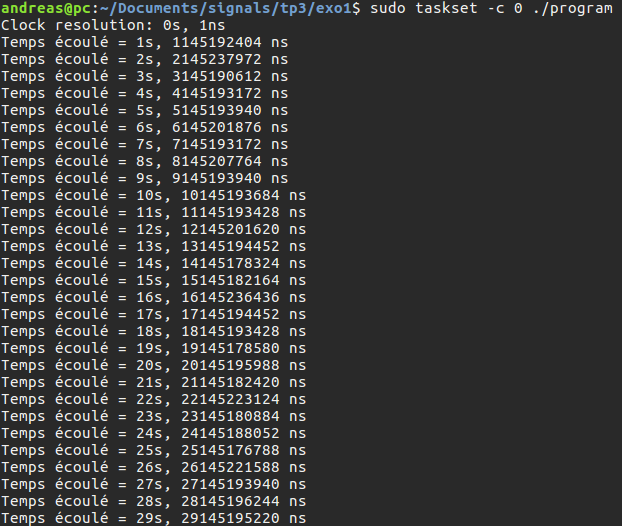
\includegraphics[width=\linewidth]{exo1.png}
  \caption{Exemple d'exécution de l'exercice 1}
  \label{fig:exo1}
\end{figure}

La figure \ref{fig:exo1} montre un exemple d'exécution du premier exercice.

On peut observer que la précision est bien plus faible que la nanoseconde annoncée par \textit{clock\_getres()}, mais qu'elle est plutôt de l'ordre de la milliseconde.

\section*{\underline{Exercice 2} :}

Dans cette partie chaque question aura son sous-dossier. Le code qui a changé est délimité par les balises \textit{// ADDED}.
\subsection*{Question 1 :}

\begin{figure}
  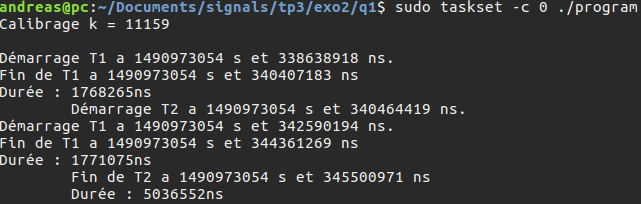
\includegraphics[width=\linewidth]{2-1.png}
  \caption{Exemple d'exécution de la première question}
  \label{fig:2.1}
\end{figure}

La figure \ref{fig:2.1} montre un exemple d'exécution. On peut aussi observer une préemption se produire lorsque T2 démarre et que T1 prends la main pendant toute la durée de son exécution.

\subsection*{Question 2 :}

\begin{figure}
  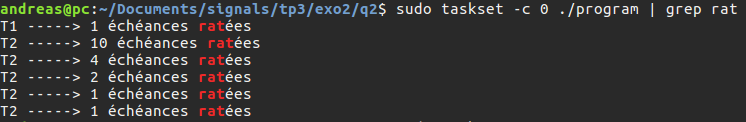
\includegraphics[width=\linewidth]{2-2.png}
  \caption{Exemple d'échéances ratées}
  \label{fig:2.2}
\end{figure}

la figure \ref{fig:2.2} montre un exemple d'exécution. Le nombre d'échéances ratées dépends largement du calibrage et du taux d'utilisation du processeur. L'exemple montre comment ces contraintes font que même T1 peut rater des échéances, alors que T2 devrait normalement être le seul à en faire.

\subsection*{Question 3 :}

Les résultats sont bien meilleurs : cela s'explique par le fait que \textit{printf()} soit très coûteux, et que les appels successifs à cette fonction va ralentir notre programme et ainsi fausser nos résultats.

\subsection*{Question 4 :}

La solution que j'ai choisie pour éliminer les appels à \textit{printf()} consiste à créer un autre processus qui va se charger d'afficher les chaînes de caractères qu'il aura reçu d'une file de messages.

\subsection*{Question 5 :}

Ajout une tâche avec une capacité égale à 6 et une période égale à 8 de plus faible priorité ne sera pas ordonnançable.

En effet, on peut utiliser le test RMA pour voir que la valeur est tellement importante qu'on peut conclure que ce ne sera pas ordonnançable sans avoir besoin de faire le test RMA étendu :

$$
\frac{2}{4} + \frac{4}{6} + \frac{6}{8} = 1.91
$$

De plus, on voit que le processeur est constamment occupé par T1 et T2 dans les 8 premières secondes d'exécution du programme vu que T1 (de plus haute priorité) va être exécuté pendant 4 unités de temps et que T2 va occuper les 4 unités restantes.

\begin{figure}
  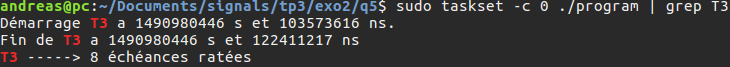
\includegraphics[width=\linewidth]{2-5.png}
  \caption{Exemple de T3 qui parvient tant bien que mal à s'exécuter dans un programme non ordonnançable}
  \label{fig:2.5}
\end{figure}

Néanmoins, on peut voir T3 s'exécuter, comme dans la figure \ref{fig:2.5}.
%----------------------------------------------------------------------------------------


\end{document}